\documentclass[10pt, xcolor=table]{beamer}
%\usetheme{Boadilla}
%\usecolortheme{beaver}
%\usepackage[latin1]{inputenc}
%\useoutertheme{split}
\setbeamertemplate{navigation symbols}{}
\usefonttheme[onlymath]{serif}
\usepackage[export]{adjustbox}
\usepackage{amsmath}%
%\usepackage[table]{xcolor}
\usepackage{amsthm}%
\usepackage{amsfonts}%
\usepackage{amssymb}%
\usepackage[algo2e]{algorithm2e}
\usepackage{algorithmic}
\usepackage{algorithm}
\usepackage{tikz}
\usepackage[english]{babel}
\usepackage{amsmath, amssymb}
\usepackage{verbatim}
\usepackage{mathrsfs}
%\usepackage{epstopdf}
\usepackage{graphicx}
%\mode<presentation>
%{
%	\usetheme{CambridgeUS}
%	\usecolortheme{dolphin}
%	\usecolortheme{rose}
%	\setbeamercovered{transparent}
%}
\newcommand{\mrel}{\mathrel{\bigcirc}}
%\usepackage[onehalfspacing]{setspace}
%\setbeamertemplate{footline}[frame number]
\DeclareMathOperator*{\Bigcdot}{\scalerel*{\cdot}{\bigodot}}
% Macros
\def\a{\alpha} \def\b{\beta} \def\c{\gamma} \def\d{\delta} \def\r{\rho}
\def\e{\epsilon} \def\ve{\varebsilon} \def\k{\kappa} \def\p{\pi} \def\th{\theta}
\def\l{\lambda} \def\m{\mu} \def\s{\sigma} \def\t{\tau} \def\w{\omega} \def\z{\zeta}
\def\D{\Delta} \def\G{\Gamma} \def\W{\Omega} \def\P{\Phi} \def\L{\Lambda}
\def\bdm{\begin{displaymath}} \def\edm{\end{displaymath}}
\def\bni{\begin{itemize}} \def\ei{\end{itemize}}
\def\bnen{\begin{enumerate}} \def\een{\end{enumerate}}
\def\fa{\forall}
\def\be{\begin{equation}} \def\ee{\end{equation}}
\def\fn{\footnote} \def\bn{\begin} \def\nit{\noindent}
\def\iff{\textit{~if and only if~~}}
\renewcommand*{\thefootnote}{\fnsymbol{footnote}}
% THEOREMS -------------------------------------------------------
\newtheorem{thm}{Theorem}%[section]
\newtheorem{cor}[thm]{Corollary}
\newtheorem{lem}[thm]{Lemma}
\newtheorem{prop}[thm]{Proposition}
\newtheorem{claim}{Claim}
\theoremstyle{definition}
%\newtheorem{defn}[thm]{Definition}
\theoremstyle{remark}
\newtheorem{rem}[thm]{Remark}
%%\numberwithin{equation}{section}

\newcommand{\N}{\mathbb{N}}
\newcommand{\Z}{\mathbb{Z}}
\newcommand{\R}{\mathbb{R}}
\newcommand{\ls}{\left\{}
\newcommand{\rs}{\right\}}


\title[Interaction-Partitioned Topic Model (IPTM)]{ \vspace{-.25cm} \\ A Network Model for \\Dynamic Textual Communications \\with Application to
	Government Email Corpora}
\author[\quad B. Kim, A. Schein, B. Desmarais and H. Wallach\quad]{
Bomin Kim\textsuperscript{1}\and
\quad Aaron Schein\textsuperscript{3}\and\\
		Bruce Desmarais \textsuperscript{1}\and Hanna Wallach\textsuperscript{2,3}}
\institute{\textsuperscript{1} The Pennsylvania State University \and \textsuperscript{2} Microsoft Research NYC \and \textsuperscript{3} University of Massachusetts Amherst}


\newenvironment{changemargin}[2]{%
  \begin{list}{}{%
    \setlength{\topsep}{0pt}%
    \setlength{\leftmargin}{#1}%
    \setlength{\rightmargin}{#2}%
    \setlength{\listparindent}{\parindent}%
    \setlength{\itemindent}{\parindent}%
    \setlength{\parsep}{\parskip}%
  }%
  \item[]}{\end{list}}

\begin{document}

\begin{frame}
  \titlepage
  \begin{center}
   \begin{tabular}{cc}
\hspace*{-.2in} \tiny \begin{minipage}{3.5in}
Work supported by NSF grants SES-1558661, SES-1619644, SES-1637089, and CISE-1320219)\\ ~\\~\\~\\~\\
\end{minipage}
& 
\includegraphics[scale=.05]{figures/NSF_Logo.PNG}
\end{tabular}
\end{center}
\end{frame}

\begin{frame}{Motivation}
\large
\begin{itemize}
\item Many networks have ties that are attributed with text:
  \vspace{0.1cm}
\begin{itemize}
\item International treaties, legislative cosponsorship, online discussions
\end{itemize}

\begin{center}
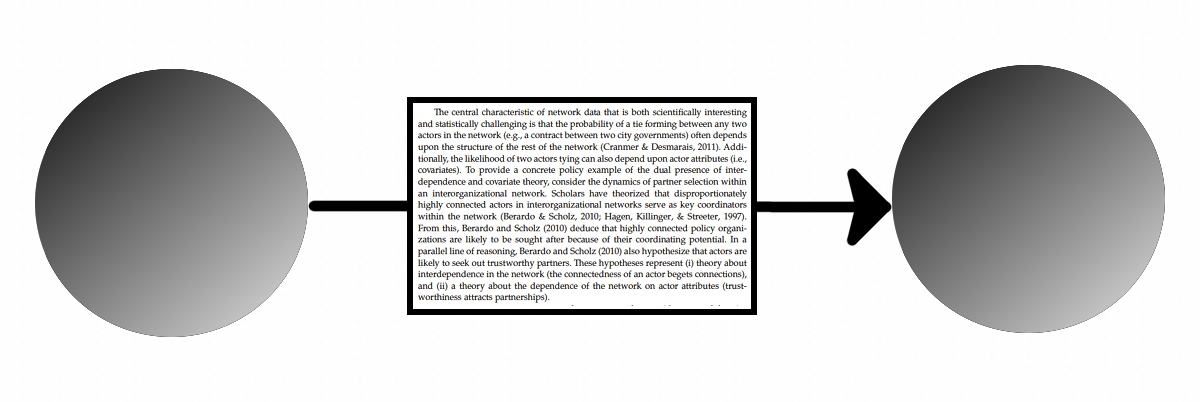
\includegraphics[scale=.15]{figures/tieWords}
\end{center} \vspace{-.1cm}
\item Network models can't account for text
\vspace{.3cm}
\item Models for text either can't account for ties or only account
  for simplistic network structure
\end{itemize}
\end{frame}

\begin{frame}{Interaction-Partitioned Topic Model (IPTM)}
\large
	\bni
	\item Model for networks with timestamped, text-valued ties
	\vspace{0.2cm}
	\item Draws on ideas from two existing models:
          \vspace{0.1cm}
	\begin{itemize}
	 \item Latent Dirichlet allocation (LDA) for topic-based
           document content
	  \item Dynamic exponential random graph model (ERGM) for ties
	  \end{itemize}
        \vspace{0.4cm}
\item \textit{Who communicates with whom about what, and when?}
  \ei
\end{frame}

\begin{frame}{Generating Content: LDA (Blei et al., 2003)}
\bni
\begin{minipage}{0.7\linewidth}
\item For each topic $k =1,...,K$:\vspace{0.2cm}
	\begin{itemize}
		\item Draw a distribution over vocabulary:
                  $\boldsymbol{\phi}_k \sim \mbox{Dir}(\beta,
                  (\frac{1}{V}, \ldots, \frac{1}{V}))$\vspace{0.2cm}

		\end{itemize}
		\vspace{0.2cm}
	\end{minipage}
	\begin{minipage}{0.25\linewidth}
			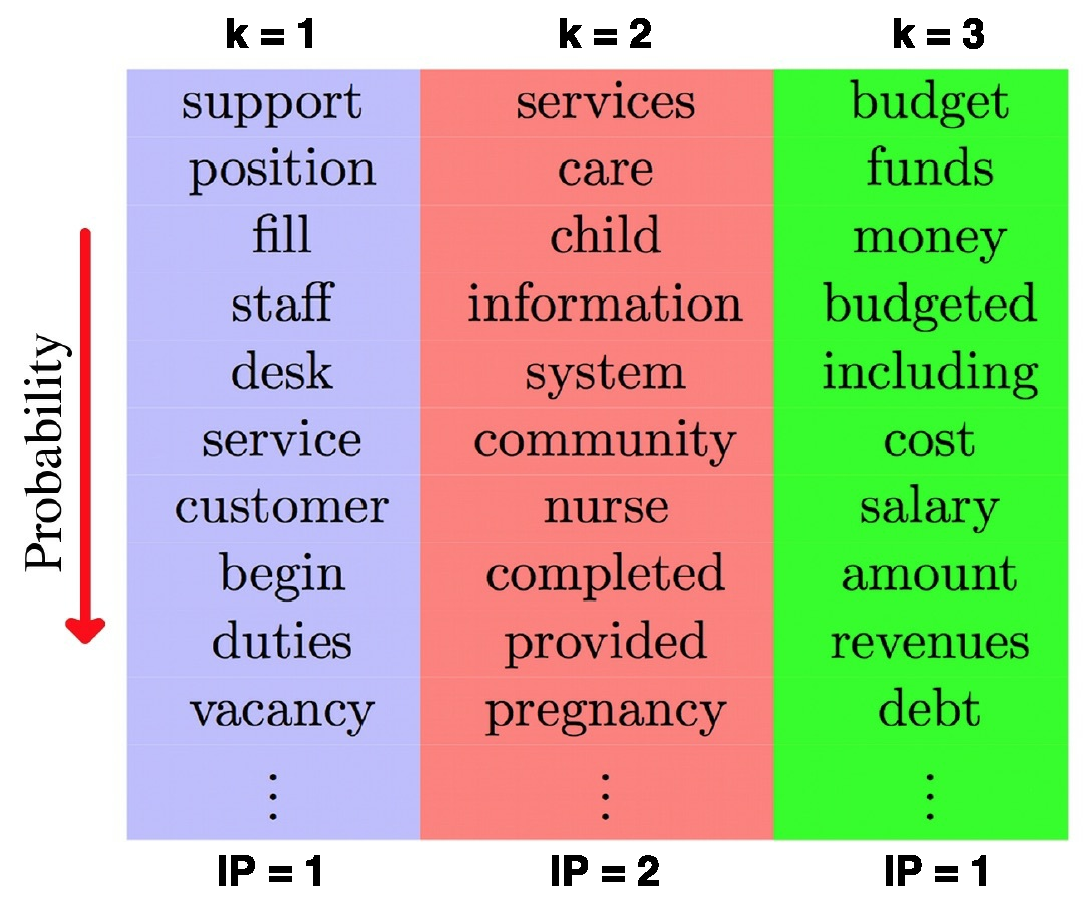
\includegraphics[width=1\textwidth]{figures/word.pdf}
				\vspace{0.2cm}
		\end{minipage}
			\begin{minipage}{0.68\linewidth}
				\item For each email $d =1,...,D:$ \vspace{0.2cm}
		\begin{itemize}
					\item Draw a distribution over
                                          topics:
                                          $\boldsymbol{\theta}_{d}
                                          \sim \mbox{Dir}(\alpha,
                                          (m_1, \ldots, m_K))$ \\\vspace{0.1cm}
		\item For each token $n=1$ to $N_d$:\vspace{0.1cm}
		\begin{itemize}
			\item Draw a topic: $z_{dn} \sim \boldsymbol{\theta}_d$\vspace{0.2cm}
			\item Draw a word type: $w_{dn} \sim \boldsymbol{\phi}_{z_{dn}}$
		\end{itemize}
			\end{itemize}
		\end{minipage}
		\begin{minipage}{0.3\linewidth}
	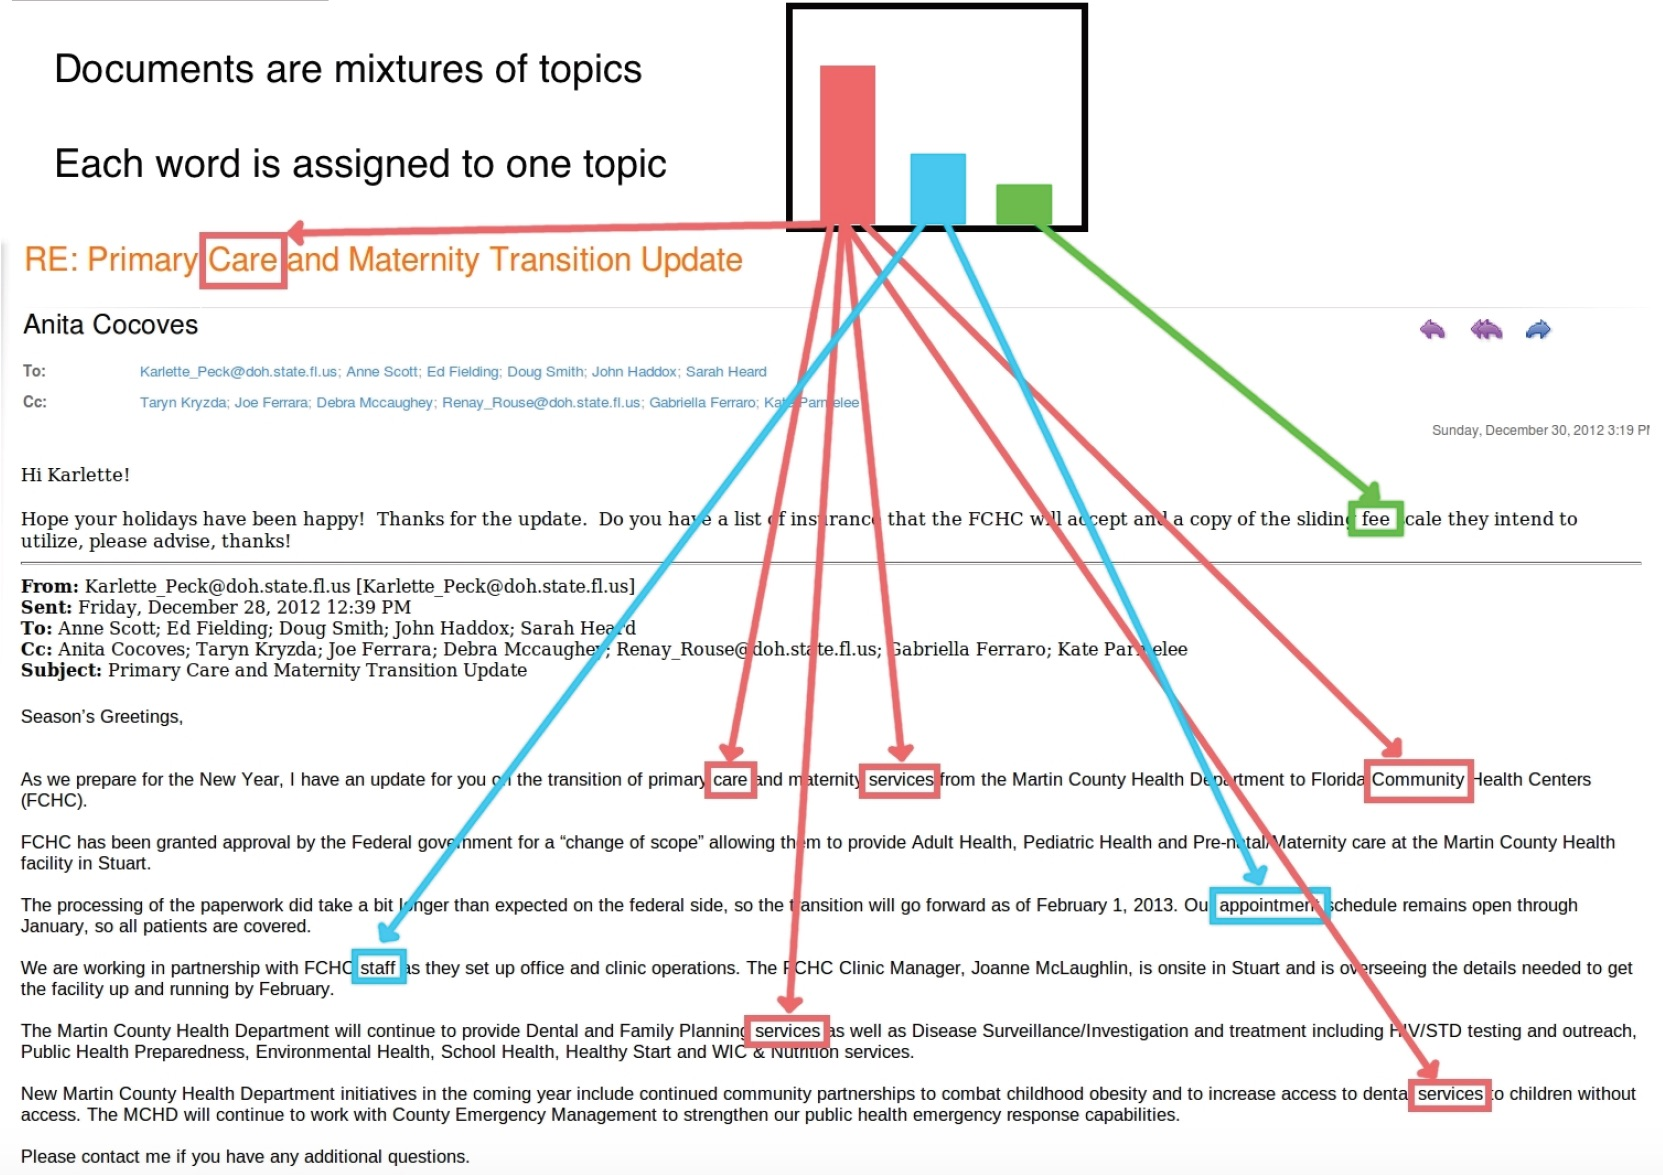
\includegraphics[width=1.05\textwidth]{figures/LDAimage.jpeg}
		\end{minipage}
		\vspace{0.2cm}
\ei
\end{frame}

\begin{frame}{Key Idea: Interaction Patterns}
\bni
\item Different topics
 associated with different interaction patterns
\item[]

\item For each topic $k =1,...,K$:\vspace{0.2cm}
	\begin{itemize}
		\item Assign topic $k$ to an interaction pattern:
                  $l_k \sim \mbox{Unif}(1, C)$
		\end{itemize}
		\vspace{0.2cm}

\item For each email $d =1,...,D$: \vspace{0.2cm}

				\begin{itemize}\item Calculate distribution over interaction patterns:
		 \footnotesize\begin{equation*}
		\pi_{dc} = \frac{\sum_{k : l_k=c} N_{dk}}{N_d}
		\end{equation*}\normalsize
	\end{itemize}
\ei
\end{frame}

\begin{frame}{Generating Ties and Timestamps}
\large
\begin{itemize}
\item Continuous-time process \vspace{.2cm}
\item Ties predicted using dynamic network features:
\begin{itemize}
\item Popularity, activity
\item Repetition, reciprocity
\item Transitivity
\end{itemize} \vspace{.1cm}
\item Author determines recipients and timestamp
  \vspace{.2cm}
\item Innovative approach to modeling multiple recipients
\end{itemize}


\end{frame}

\begin{frame}{Generating Hypothetical Authors and Recipients}
		\begin{itemize}
		\item [1.] For each author $i \in \{1,...,A\}$ and recipient $j \in \{1,...,A\}$ ($i \neq j$), calculate the stochastic indensity between $i$ and $j$:
	%	\footnotesize
			\begin{align*}\nu_{idjc} &= \mbox{exp}({\boldsymbol{b}_c}^{\top}\boldsymbol{x}_{idjc})\\
                          \lambda_{idj} &=\sum_{c=1}^{C} \pi_{dc}\, \nu_{idjc}
			\end{align*}\normalsize
		which combines information about content and network structure\\ \vspace{0.4cm}
		\item[2.] For each author $i \in \{1,...,A\}$, draw a
                  binary vector $\boldsymbol{u}_{id}$ of length $A$
                  from a non-empty Gibbs measure (Fellows and Handcock, 2017)
	%	\footnotesize
		%\mbox{log}\big(\text{I}( \sum_{j \in \mathcal{A}_{\backslash i}} J^{(d)}_{ij} > 0 )\big) +
		\begin{equation*} \boldsymbol{u}_{id} = (u_{id1},
                  \ldots, u_{idA}) \sim
                  \mbox{Gibbs}(\delta, (\lambda_{id1}, \ldots, \lambda_{idA}))
		\end{equation*}
		\normalsize
		where $\delta$ is a real-valued value that controls
                the number of recipients\\\vspace{0.1cm}
	\end{itemize}
	\end{frame}
\begin{frame}{Generating Hypothetical Timestamps and Actual Data}
\begin{itemize}
		\item [3.] For each author $i \in \{1,...,A\}$,
                  generate a timestamp:
	%	\footnotesize
		\begin{align*}
                  \mu_{id} &= \sum_{c=1}^C \pi_{dc}\, \mbox{GeomMean}(\{
                  \nu_{idjc} \}_{j:u_{idj}= 1})\\
		\tau_{id} &\sim \mbox{Exp}(\eta\,\mu_{id})\\
                t_{id} &= t_{d-1} + \tau_{id}
		\end{align*}\normalsize
		where $\eta$ is a positive real-valued value \vspace{0.4cm}
		\item[4.] Select the actual author, recipients, and timestamp:
		%\footnotesize
			\begin{align*}
		a_d &= \mbox{argmin}_{i}(t_{id})\\
		\boldsymbol{y}_d &= \boldsymbol{u}_{a_d d}\\
		t_d &= t_{a_d d}
		\end{align*}
		\normalsize
\end{itemize}
 %\begin{figure}
 %	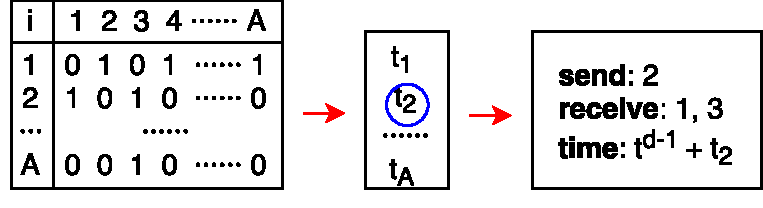
\includegraphics[width=0.57\textwidth]{figures/tie.pdf}
 %\end{figure}
\end{frame}

\begin{frame}{Generating Ties and Timestamps}

	\begin{figure}
		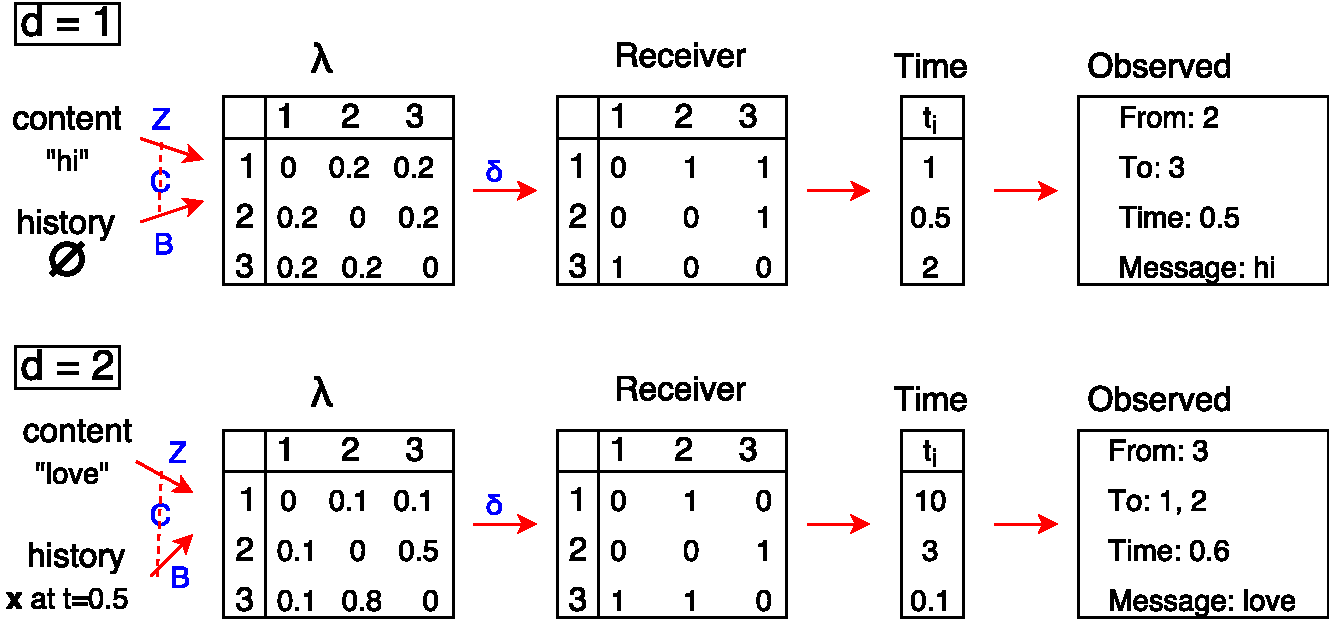
\includegraphics[width=0.9\textwidth]{figures/summary.pdf}
	\end{figure}	\vspace{0.1cm}

\end{frame}

\begin{frame}{Network Features (Perry and Wolfe, 2012)}

\large
\begin{itemize}
\item Features capture different types of interaction: popularity,
  activity, repetition, reciprocity, transitivity
\end{itemize}

	 \begin{figure}
	 	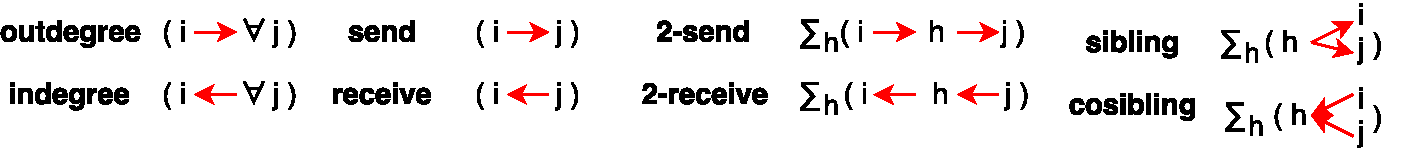
\includegraphics[height= 2cm, trim= 0cm 0cm 14cm 0cm, clip=true]{figures/netstats.pdf}\\ \vspace{-.5cm}
		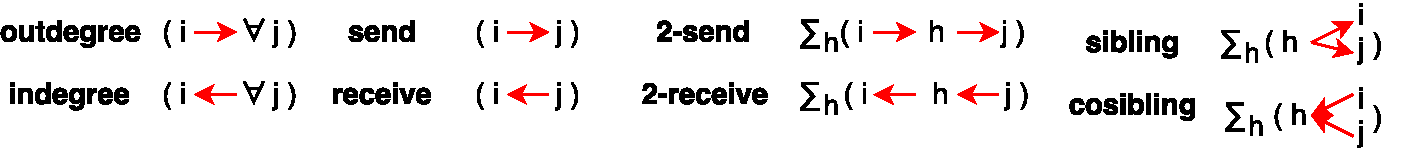
\includegraphics[height= 2cm,, trim= 10cm 0cm 0cm 0cm, clip=true]{figures/netstats.pdf}
	 \end{figure}

\end{frame}

\begin{frame}{Dynamic Network Features}


\begin{itemize}
\item To form $\boldsymbol{x}_{idjc}$, consider 3 time intervals prior
  to $t^{+}_{d-1}$:\vspace{0.1cm}
  \begin{itemize}
    \item 3--16 days, 1--3 days, 0--1 days
  \end{itemize}
  \vspace{0.2cm}

\item For each interval, compute each network feature focusing on
  emails in that interval: 24 dynamic network features in
  $\boldsymbol{x}_{idjc}$

\end{itemize}
  \vspace{0.2cm}
\centering
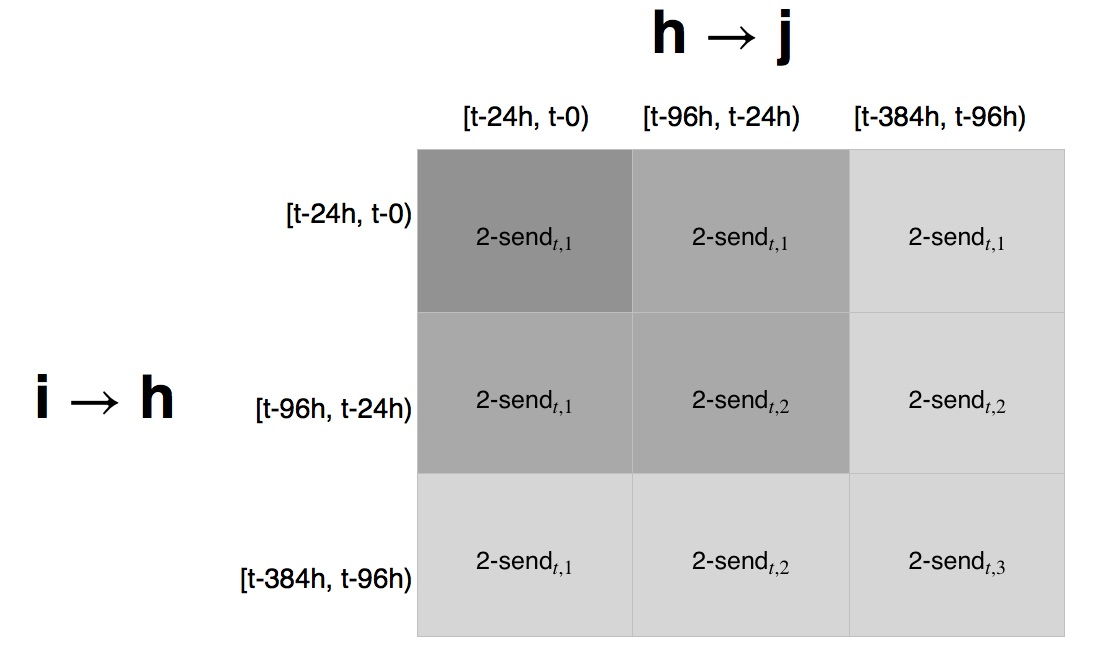
\includegraphics[scale=.15]{./figures/triadtable}

\end{frame}


\begin{frame}{Inference}

%\begin{itemize}
%\item Take a Bayesian approach to inference (of course)
%\end{itemize}
  	\begin{center}
  		\scalebox{.9}{
 	 \begin{minipage}{1\linewidth}\begin{algorithm}[H]
\SetAlgoLined
	 	\caption{MCMC: Metropolis-Hastings within Gibbs}
	 	Initialize latent variables\\
	 	\For{o=1 to O}{
	 				Sample
                                        \textcolor{blue}{token--topic
                                          assignments} $z_{dn}$\\
	 			Sample
                                \textcolor{blue}{topic--interaction
                                  pattern assignments} $l_k$\\
	 				Sample
                                        \textcolor{blue}{hypothetical
                                          author--recipient set pairs}
                                        $\boldsymbol{u}_{ad}$\\
	 		 				Sample
                                                        \textcolor{blue}{coefficients} $\boldsymbol{b}_c$
                                                        using Metropolis-Hastings \\
	 			Sample \textcolor{blue}{recipient parameter} $\delta$ using Metropolis-Hastings\\
	 			Sample \textcolor{blue}{timestamp parameter} $\eta$ using Metropolis-Hastings
	 	}
	 \end{algorithm}
	\end{minipage}}
	 	\end{center}
\end{frame}


\begin{frame} \frametitle{Getting it Right: Testing Math and Code
    (Geweke, 2004)}

\begin{itemize}
\item {\em Generate forward samples}:
\begin{enumerate}
\item Draw latent variables from priors
\item Draw synthetic data conditioned on latent variables
  \item Repeat 1 and 2 many times
\end{enumerate} \vspace{.2cm}
\item {\em Backward samples}:
\begin{enumerate}
\item Start with a forward sample
\item Draw latent variables from posterior using inference code
\item Draw synthetic data conditioned on latent variables
\item Repeat 2 and 3 many times
\end{enumerate} \vspace{.2cm}
\item Forward samples and backward samples should match
\end{itemize}


\end{frame}

\begin{frame} \frametitle{Getting it Right Results}
\begin{center}
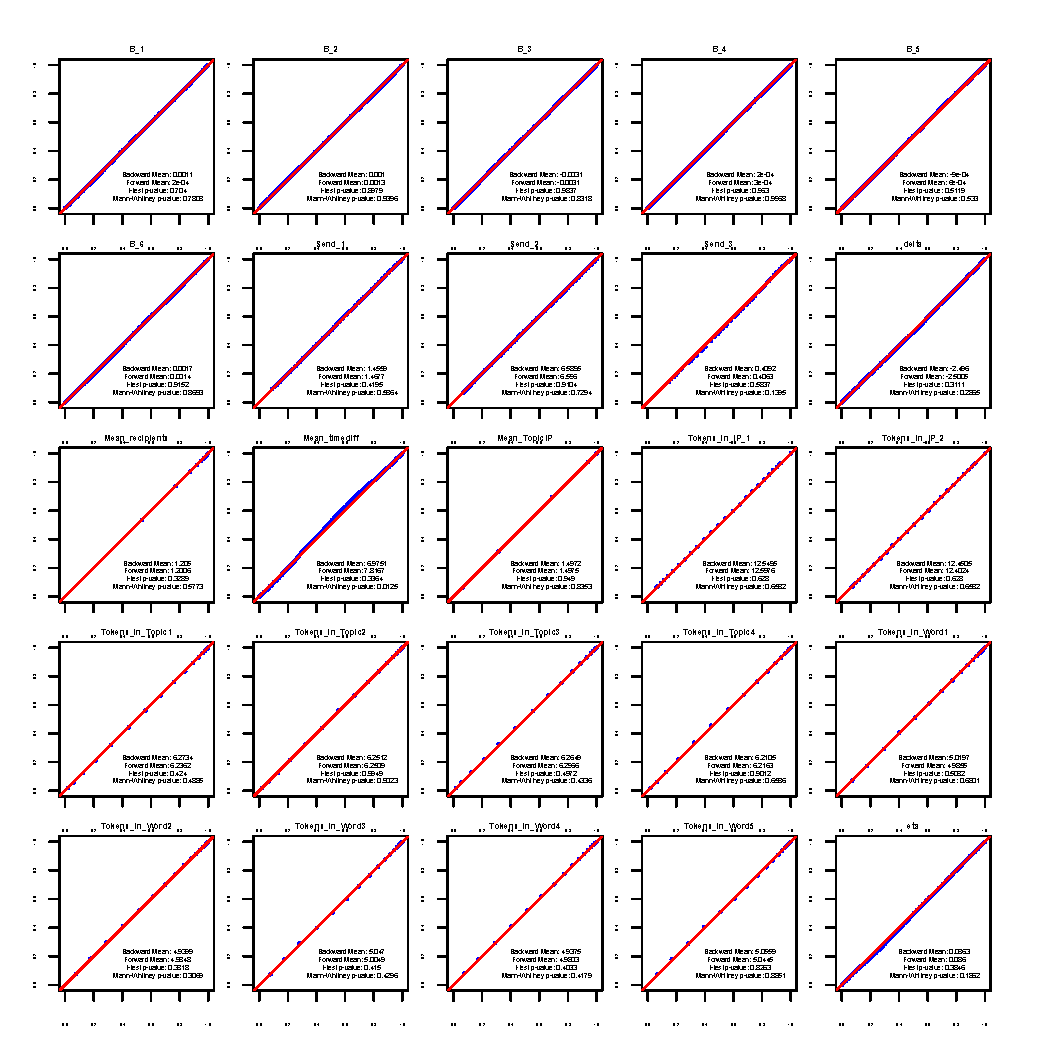
\includegraphics[width=0.6\textwidth]{./figures/GiReta}
\end{center}
\end{frame}

\begin{frame}{NC Email Corpus: Dare County}
\begin{center}
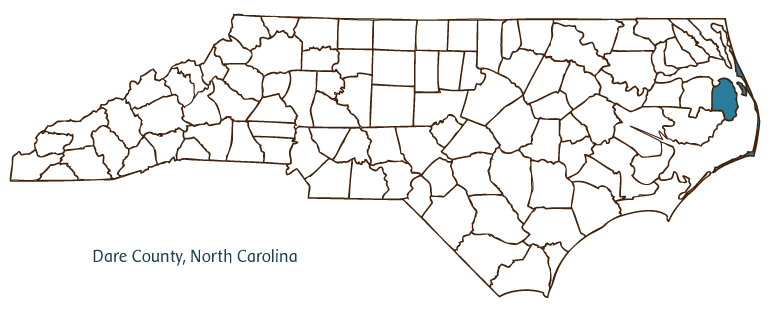
\includegraphics[width=0.6\textwidth]{figures/dare.png}
\end{center}
 \begin{itemize}
 \item $D = 2,210$ emails
\item  $A = 27$ department managers
\item  $V = 2,907$ words in vocabulary
\item Covers 3 months (September 1 to November 30) in 2012:
  \vspace{0.1cm}
\begin{itemize}
  \item Hurricane Sandy: October 26 to October 30
    \end{itemize}
 \end{itemize}
\end{frame}

\begin{frame}{Example Email}
  \begin{minipage}{0.7\linewidth}
\begin{itemize}
	\item From: Health\\
	\item To: County Manager\\
	\item At: 8 April 2012 8:46:00\\
	\item Content: ... A few months ago Jennifer was on call
          and Friday night she was out till 2 am and started the calls
          before 5pm, there were 2 bites at one time and then a goat
          in the highway, she took the goat to her barn because we did
          not have anywhere to keep it...
	\end{itemize}
\end{minipage}
  \begin{minipage}{0.25\linewidth}
\begin{center}
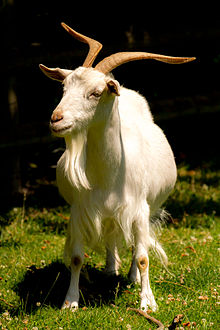
\includegraphics[width=0.90\textwidth]{figures/goat.jpg}\\
\tiny (Not the actual goat.)
\end{center}
\end{minipage}
\end{frame}


\begin{frame}{Hypotheses}
\large
\begin{itemize}
\item Personal/social topics exhibit reciprocity and transitivity \vspace{.4cm}
\item Dissemination topics don't exhibit reciprocity\vspace{.4cm}
\item Topics about Hurricane Sandy look different
\end{itemize}

\end{frame}

\begin{frame}{Data Exploration}
\begin{center}
	\begin{minipage}{0.75\linewidth}

	 	 \begin{figure}
	 	 	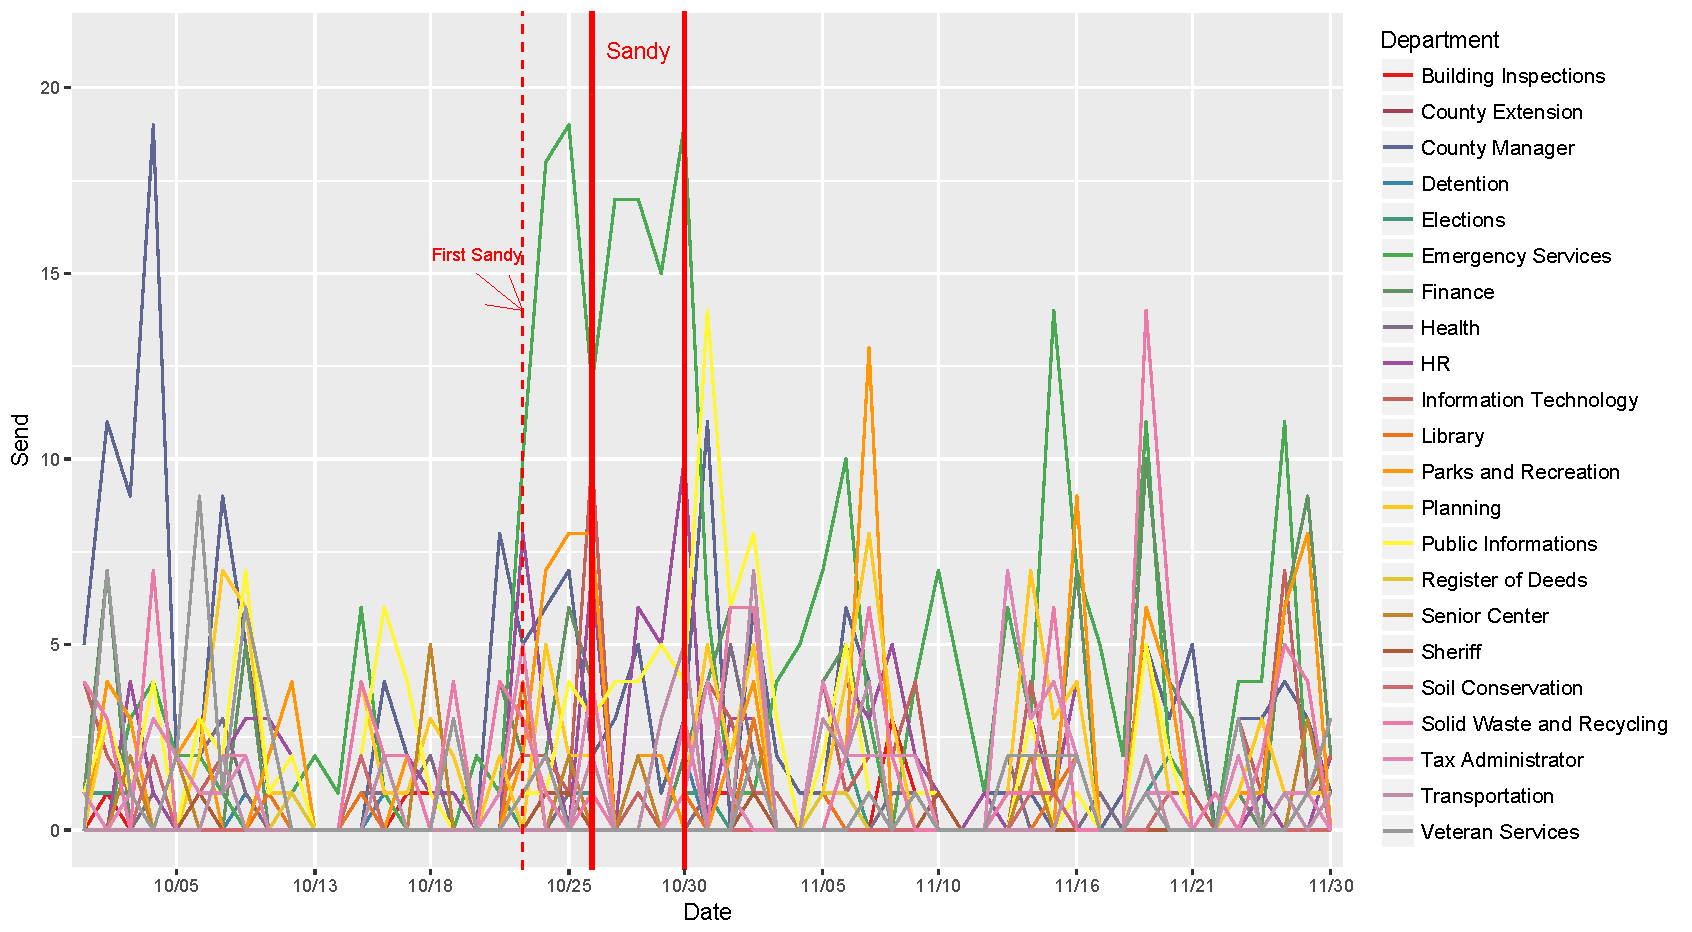
\includegraphics[width=0.5\textwidth, trim = 0cm 0cm 6cm 0cm, clip=true]{figures/DareSend.pdf}
	 	 	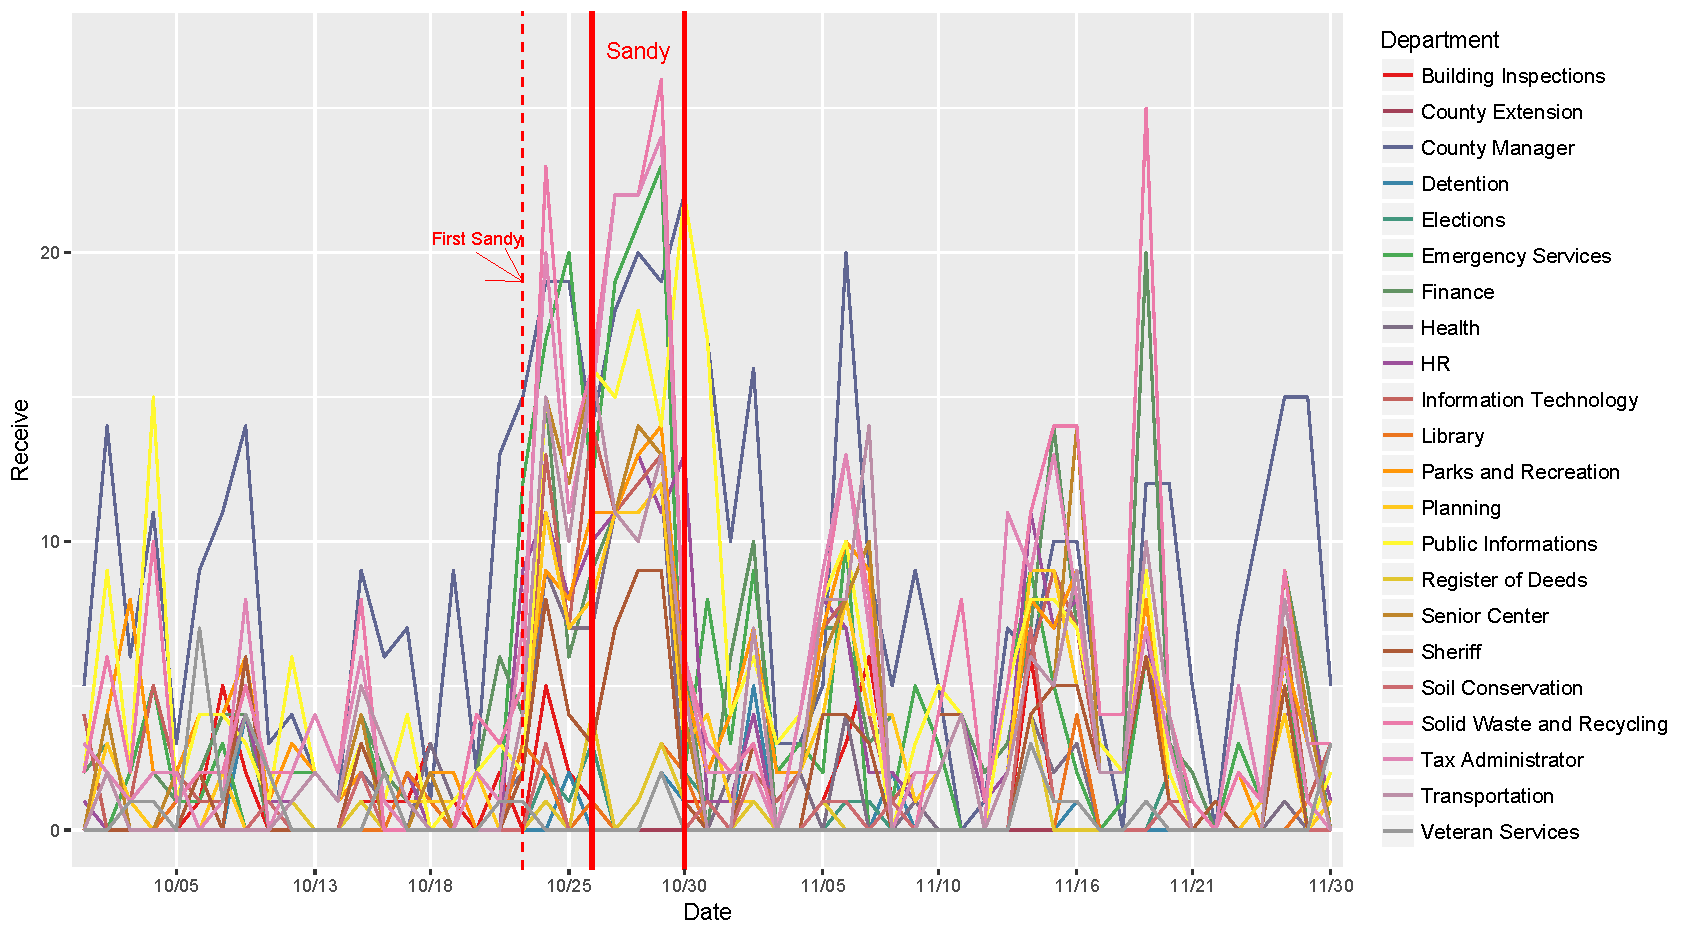
\includegraphics[width=0.5\textwidth, trim = 0cm 0cm 6cm 0cm, clip=true]{figures/DareReceive.pdf}
	 	 \end{figure}	\vspace{-.5cm}
	 \begin{figure}
	 		 	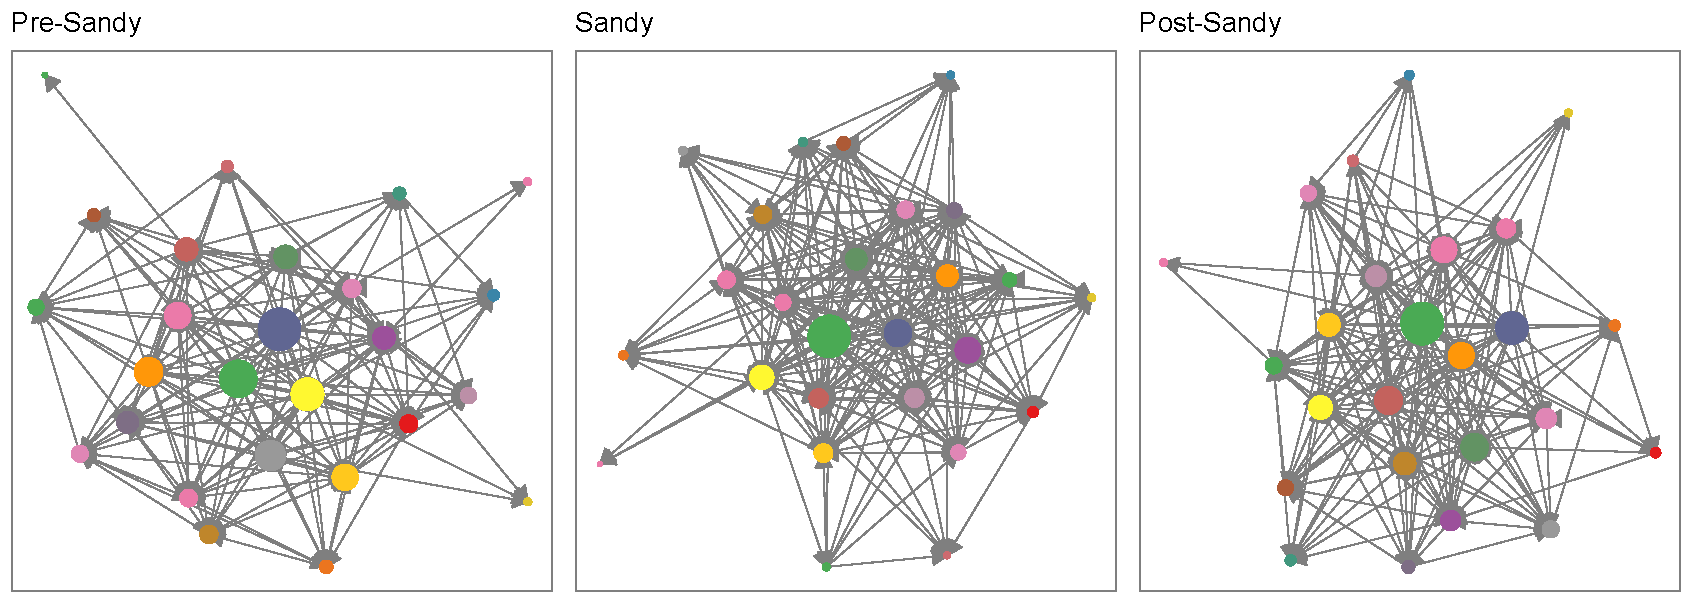
\includegraphics[width=1\textwidth]{figures/DareNetwork.pdf}
	 		 		 \end{figure}
\end{minipage}
\begin{minipage}{0.13\linewidth}
		 \begin{figure}
	 		 		 	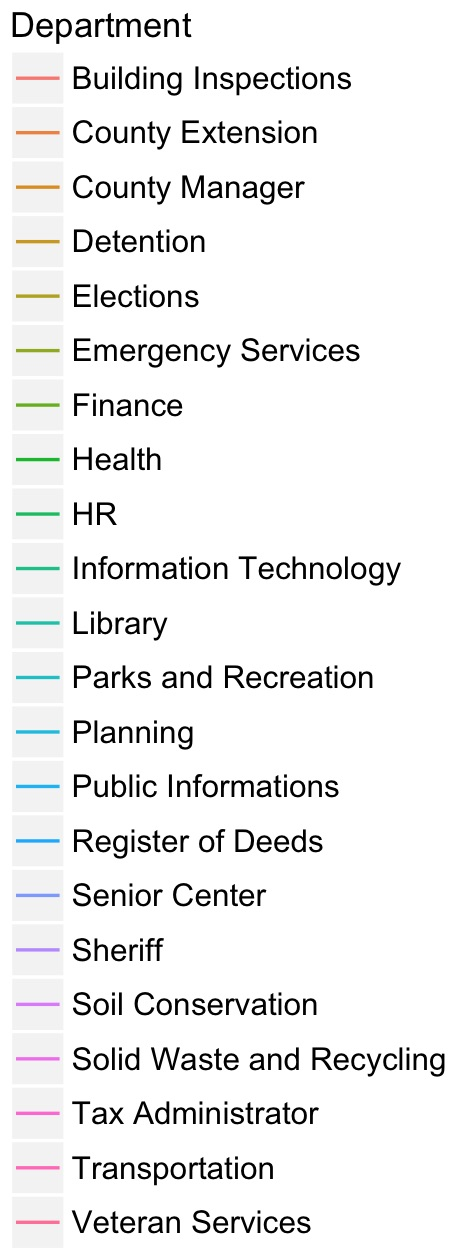
\includegraphics[width=1.25\textwidth]{figures/Dept2.jpg}
	 \end{figure}
	\end{minipage}
\end{center}
\end{frame}



 \begin{frame}{Interaction Pattern 1: Top 5 Topics}
\begin{center}
  	\scalebox{0.7}{	 	\begin{tabular}{ |c|c|c|c|c|}
  			\hline
  			\textbf{23}&   \textbf{18} &\textbf{11} &\textbf{20} &\textbf{8}  \\ \hline\hline

  		change & will &  \cellcolor{blue!25} sandy & time & services\\
  		order & \cellcolor{blue!25}  winds &  munis & hours & public \\
  		manager &  location & \cellcolor{blue!25} hurricane& monday & white\\
  		\cellcolor{blue!25} storm & \cellcolor{blue!25} beach &  position & leave & director \\
  		\cellcolor{blue!25}emergency &  \cellcolor{blue!25} hydrant & monday &employees & fyi\\
  		\cellcolor{blue!25} coastal & \cellcolor{blue!25} water & point & timesheets &tim \\
  		 statute & relocation &  power& \cellcolor{blue!25} storm & \cellcolor{blue!25} update \\
  		\cellcolor{blue!25}evacuation & mirlo & update & employee & \cellcolor{blue!25} status\\
  		\cellcolor{blue!25} track &  road & \cellcolor{blue!25} storm& tomorrow &board \\
  		couple & high & hey & work & approval\\
  		changes & moving & release& regular &wanted\\
  		well & gas & weeks & period &rec\\
  		concerns & \cellcolor{blue!25}  forecast & weekend & comp & adult\\
  		things & saturday & working&sheets &older\\
  		consistent & project & month& vacation & today\\
  		\cellcolor{blue!25} boat &  \cellcolor{blue!25} outer & problems&administrative &\cellcolor{blue!25} storm  \\
  		 misdemeanor & map & \cellcolor{blue!25} strong& operation & reminder\\
  		 program &airport & \cellcolor{blue!25} impacts & timesheet &called\\
  		 \cellcolor{blue!25} system &called &  three & personnel & sep\\
  		 powerpoint &  \cellcolor{blue!25} banks & ncdot & will &charlotte \\
  			\hline
  		\end{tabular}}
        \end{center}
\end{frame}

\begin{frame}{Example Email}
\begin{itemize}
	\item From: Public Information\\
	\item To: Emergency Services, Detention\\
	\item At: 25 Oct 2012 19:14:47\\
	\item Content:
\textcolor{blue}{ will will storm good \textcolor{black}{sure} sandy morning morning morning morning send change plan hurricane wanted copy base afternoon keep description description saturday saturday saturday saturday touch touch release signature plans prior ready duration submitted eoc running exactly activation activation released mind joint jis pasted \textcolor{black}{activate}}
	\end{itemize}
\end{frame}



 \begin{frame}{Interaction Pattern 2: Top 5 Topics}
\begin{center}
  	\scalebox{0.7}{	 	\begin{tabular}{ |c|c|c|c|c|}
  			\hline
  			 \textbf{21} & \textbf{12} &\textbf{14} &\textbf{4} &\textbf{10} \\ \hline\hline
  			library & marshall & will&board & survey\\
  			best & collins &center&meeting & request\\
  			start & drive &day& property &call \\
  			web & manteo & office&planning & sure\\
  			place & phone & great&will & people\\
  			visit &box & manager&notice &emergency \\
  			albermarle & fax &assistance&  january & thought\\
  			east & resources & problem& review & seafood\\
  			regional & director & lot&commissioners & mail\\
  			system & human & call&list & grant\\
  			voice &phr &  currently&thoughts & ncacc \\
  			librarian &policy &september& amendment &community\\
  			learning & time &early&  members &check \\
  			discovery & october &parking& dot & rodanthe\\
  			manteo & hire & received&budget & district\\
  			expressed & will & monday& building & complete\\
  			views & offices & baum&inspections &option \\
  			box & approved &questions& night &best\\
  			conversion & hour & year&text & residents\\
  			director &told&today& copy &talk\\  			\hline
  		\end{tabular}}
        \end{center}
\end{frame}


\begin{frame}{Coefficients}
	\begin{figure}
		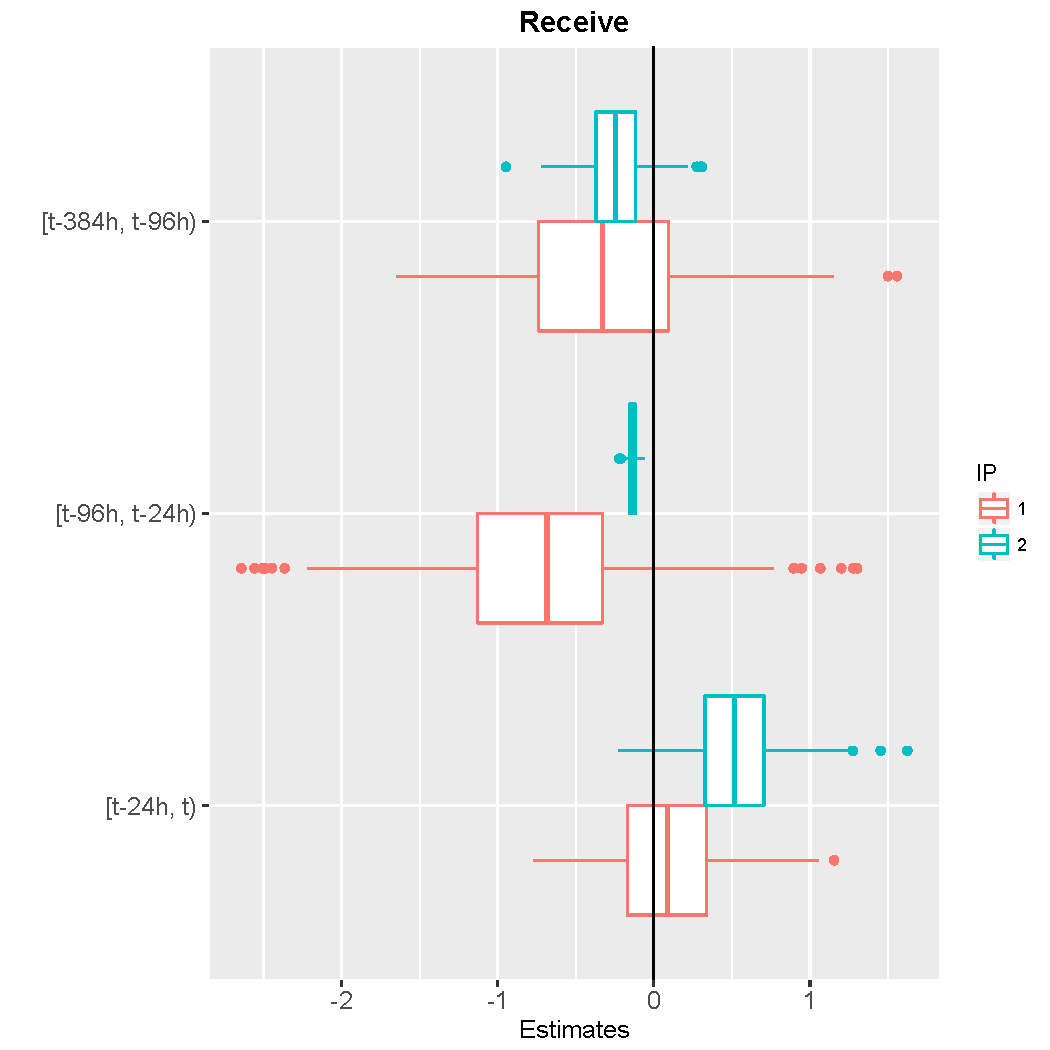
\includegraphics[width=.5\textwidth]{figures/receive.pdf} 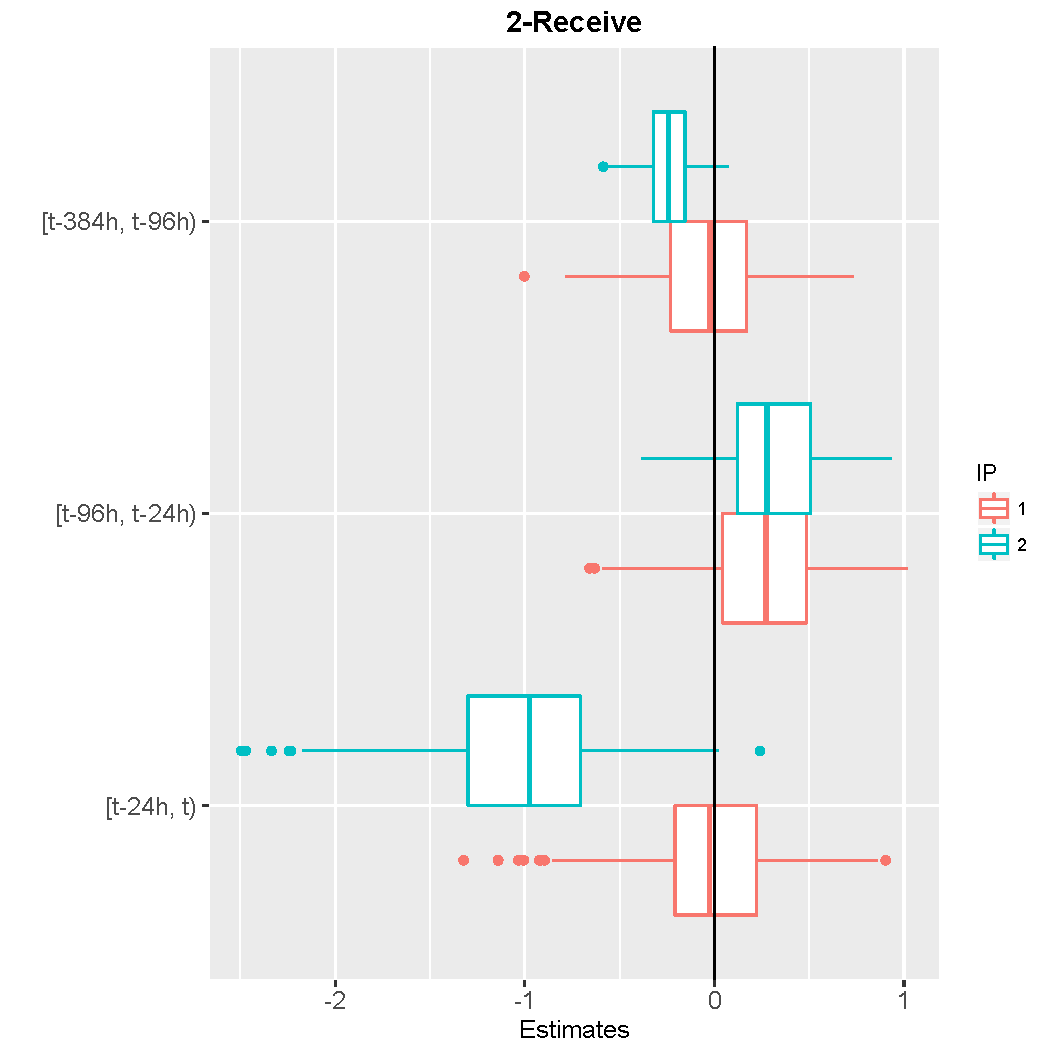
\includegraphics[width=.5\textwidth]{figures/2receive.pdf}
			\end{figure}
\end{frame}

\begin{frame} \frametitle{Predicting Ties and Timestamps}
 	\begin{center}
\scalebox{.8}{
 \begin{minipage}{1\linewidth}
\begin{algorithm}[H]
	\SetAlgoLined
	\caption{Predict ties and timestamp for next email}
	Run burn-in iterations of MCMC on emails 1 through $d-1$\\
	\For{o=1 to O}{
		Run single iteration of MCMC on emails 1 through $d-1$\\
                Initialize $a_{d}$, $\boldsymbol{y}_d$, $t_d$, and $\boldsymbol{z}_d$\\
		\For{r=1 to R}{
		Sample $a_{d}$, $\boldsymbol{y}_d$, $t_d$ conditioned on
                $\boldsymbol{z}_d$ using generative process\\
                Sample $\boldsymbol{z}_d$ from conditional posterior
		}
		Save $a_d$, $\boldsymbol{y}_d$, $t_d$, and $\boldsymbol{z}_d$
	}
\end{algorithm}
\end{minipage}
}
\end{center}
\end{frame}


\begin{frame} \frametitle{Example Results}
\begin{center}
	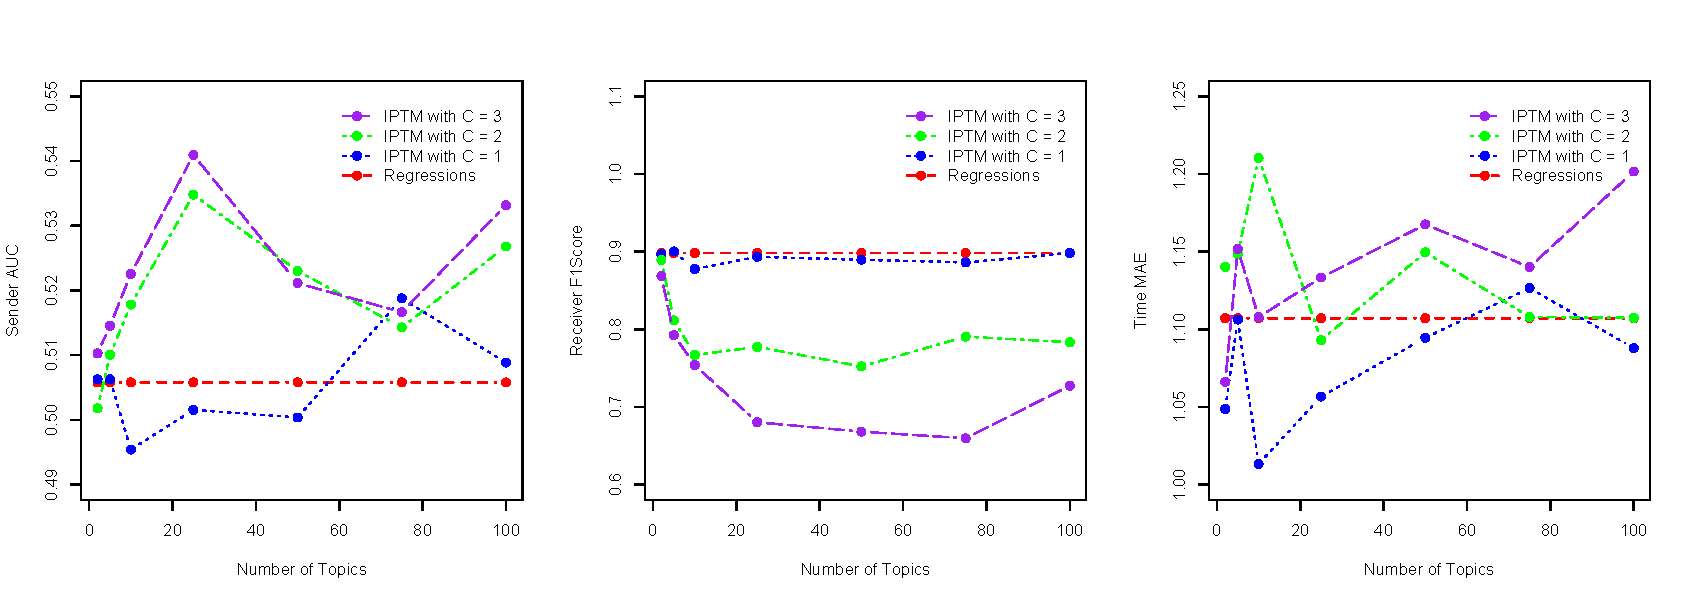
\includegraphics[width=0.85\textwidth]{figures/Dare_PPE_22.pdf}
	\end{center}
\begin{itemize}
	\item Model does poorly at predicting ties and timestamps
\end{itemize}
\end{frame}

\begin{frame} \frametitle{Posterior Predictive Checks}
\begin{center}
	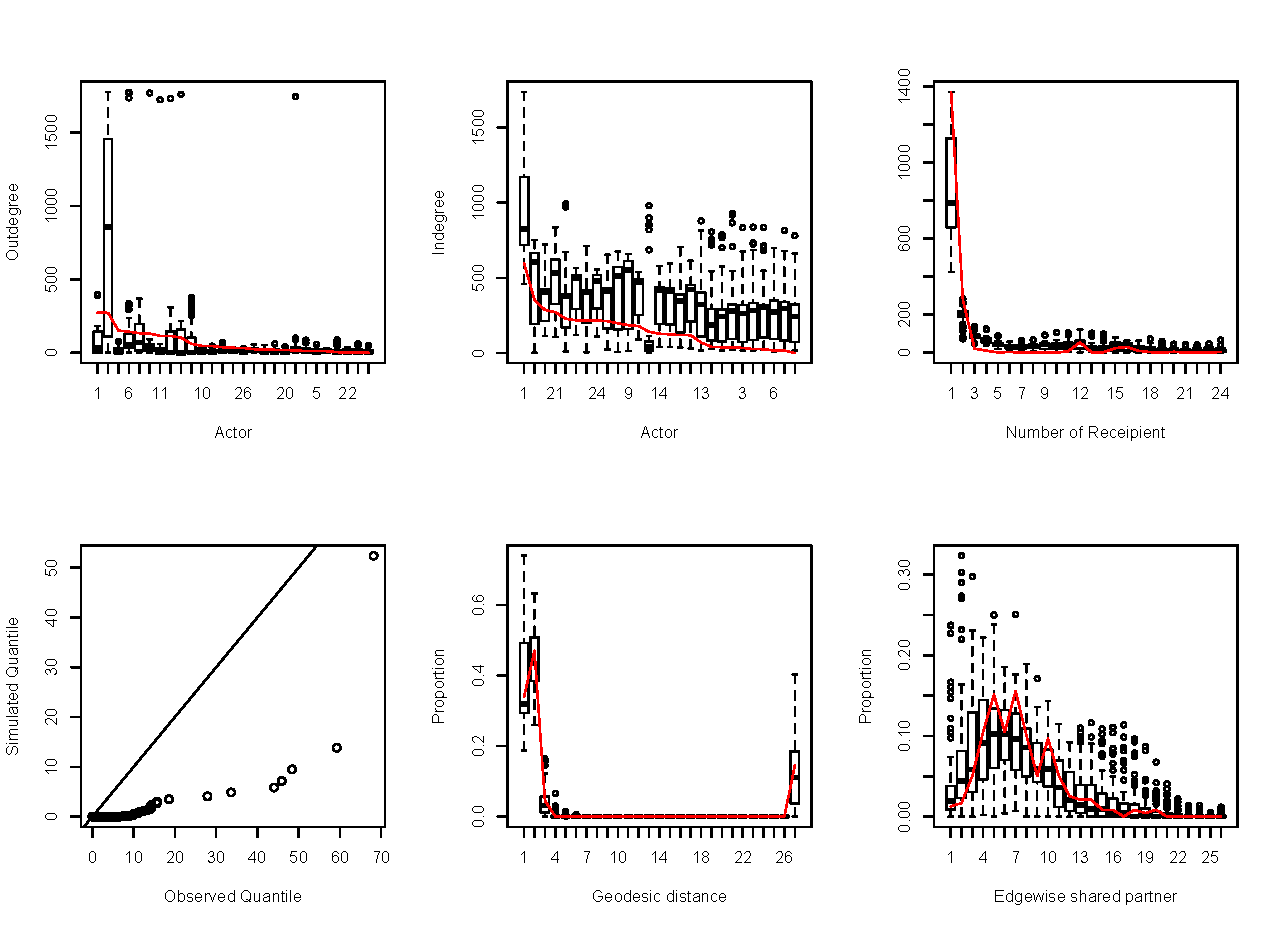
\includegraphics[width=0.85\textwidth]{figures/PPC_Dare_80.pdf}
	\end{center}
\end{frame}


\begin{frame}{To Conclude...}
  \large
 \bni
 \item Model for networks with timestamped, text-valued ties
 	\vspace{0.4cm}
 \item Many potential applications in political science
 	\vspace{0.4cm}
 	\item Developement of R package `IPTM'
 \ei
\end{frame}

\begin{frame}{I otter know the answer...}
  \begin{center}
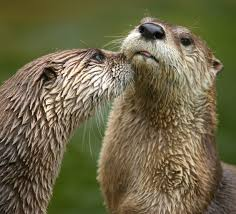
\includegraphics[width=0.65\textwidth]{figures/otter}
\end{center}
\end{frame}

\begin{frame}{I don't have the necessary koalafications...}
  \begin{center}
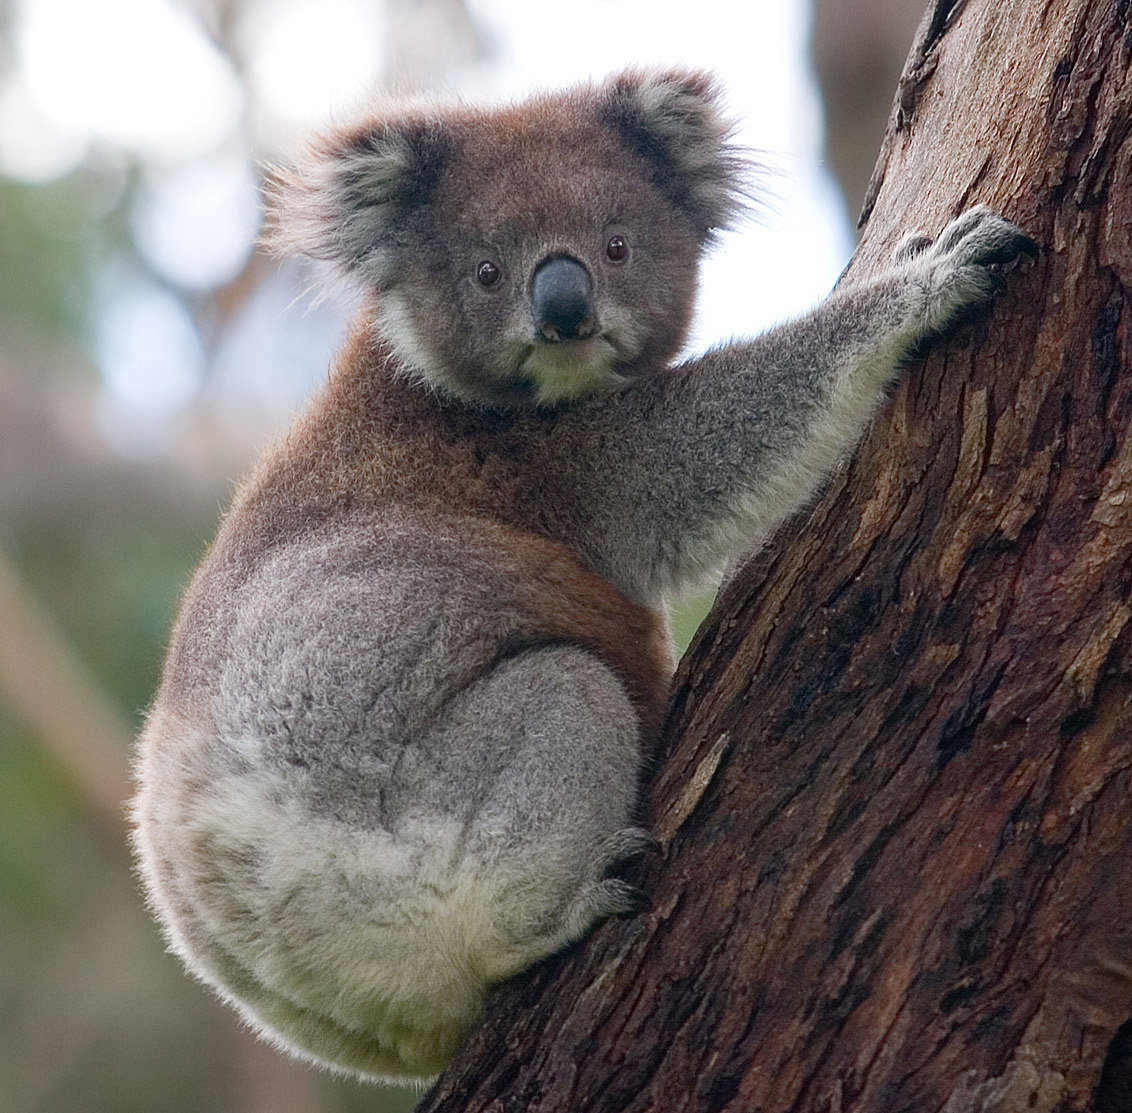
\includegraphics[width=0.6\textwidth]{figures/koala}
\end{center}
\end{frame}

\begin{frame}{If they'd gibbon me more time...}
  \begin{center}
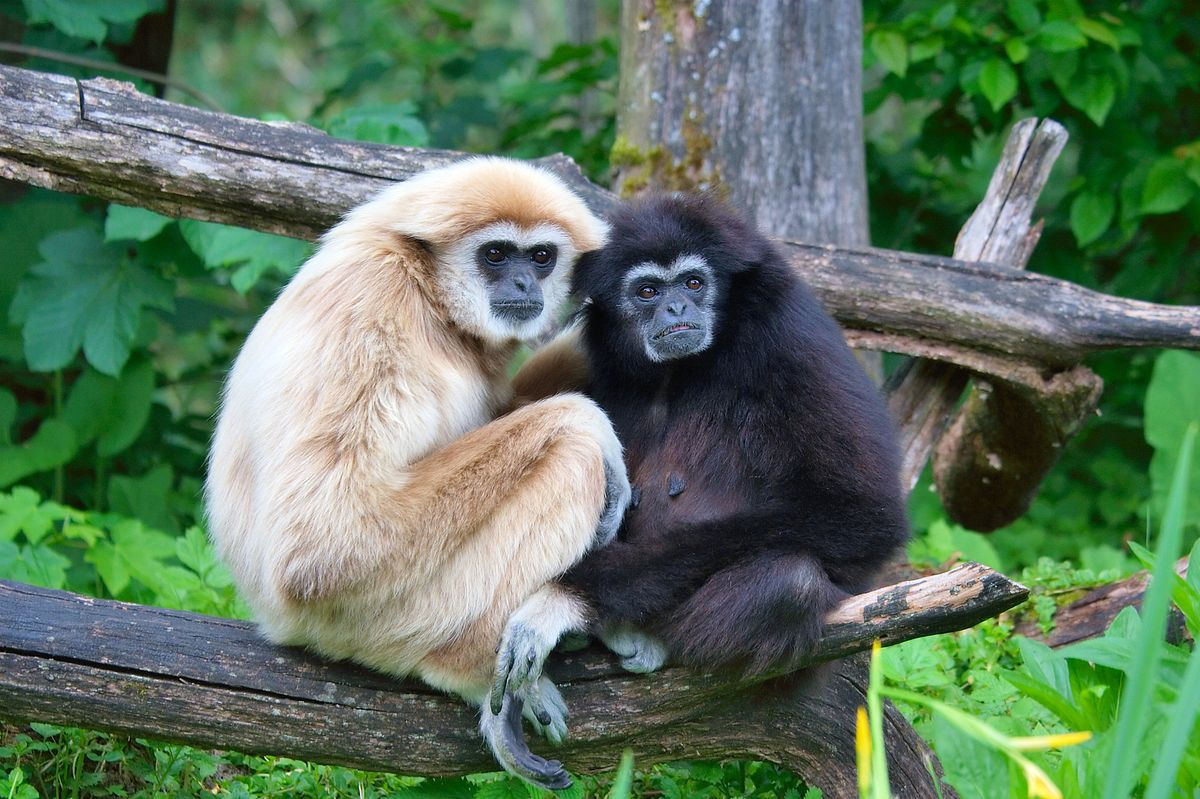
\includegraphics[width=0.85\textwidth]{figures/gibbon}
\end{center}
\end{frame}

\begin{frame}{If I'd implemented the IPTM with my bear hands...}
  \begin{center}
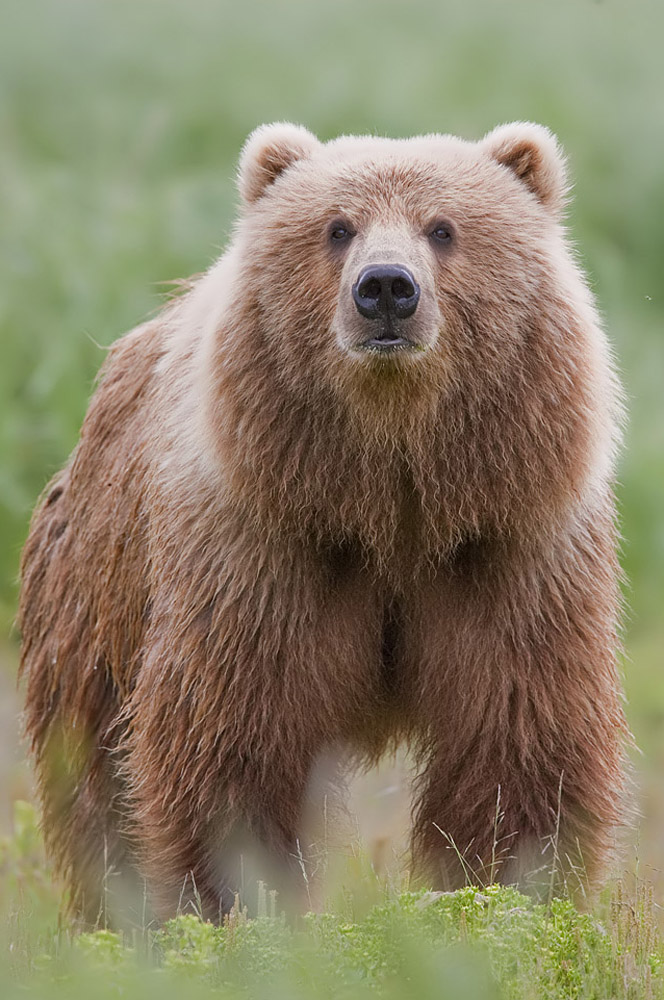
\includegraphics[width=0.4\textwidth]{figures/bear}
\end{center}
\end{frame}

\begin{frame}{I'd be lion if I said yes...}
  \begin{center}
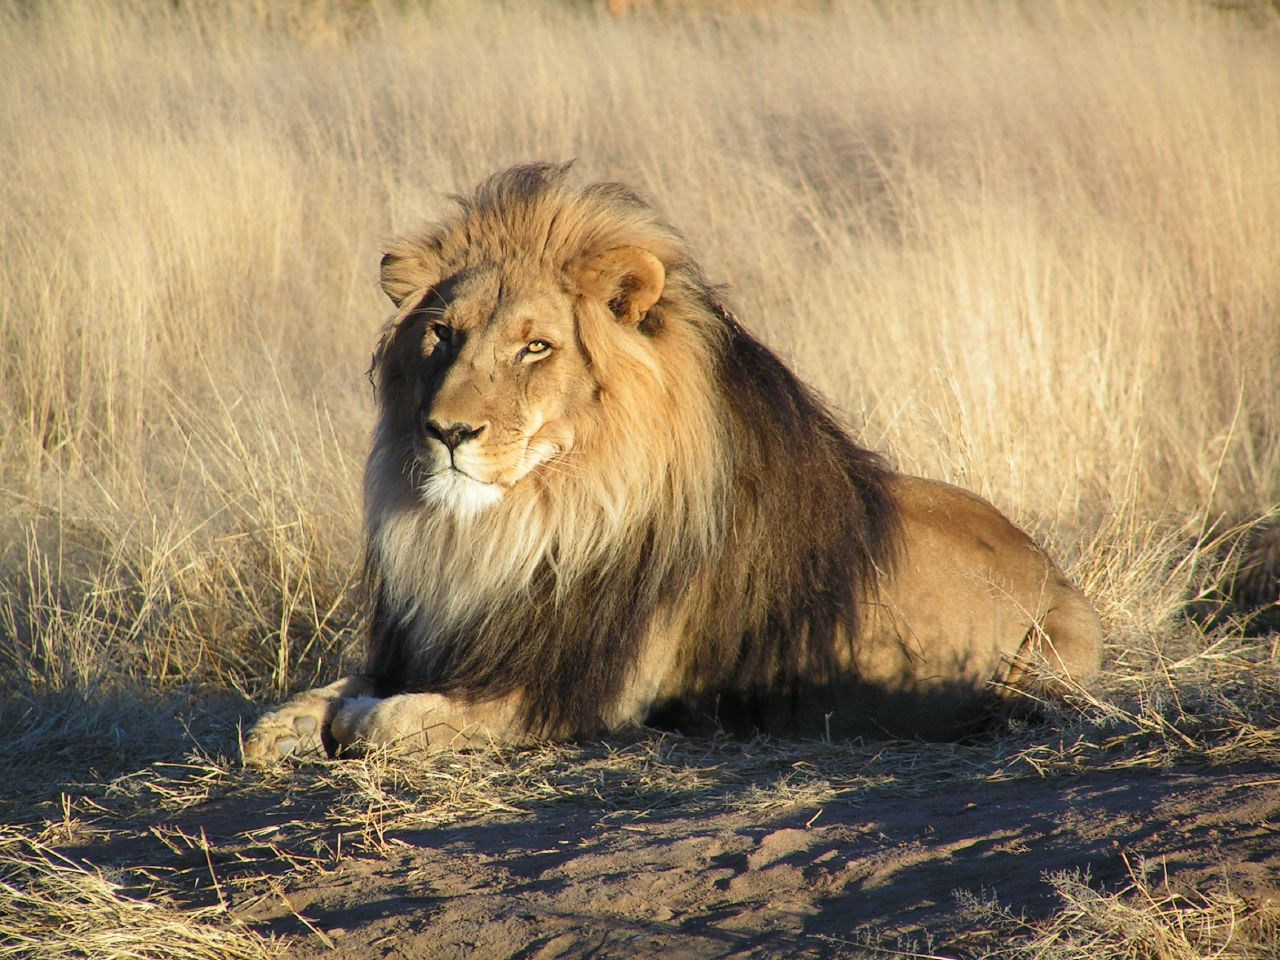
\includegraphics[width=0.75\textwidth]{figures/lion}
\end{center}
\end{frame}

\begin{frame}{Let's table bat discussion...}
  \begin{center}
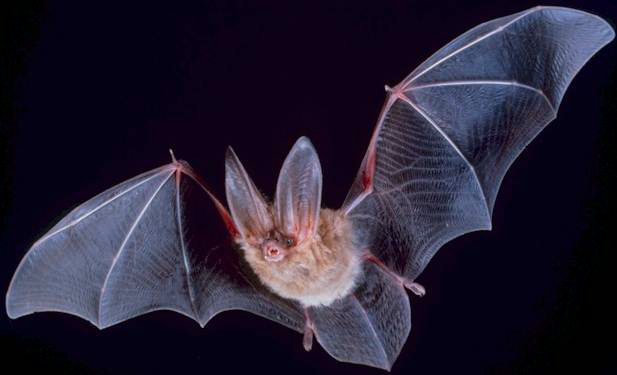
\includegraphics[width=0.85\textwidth]{figures/bat}
\end{center}
\end{frame}


\end{document}
